\documentclass[border=16pt]{standalone}

\usepackage{amsmath}
\usepackage{amssymb}
\usepackage{xcolor}
\usepackage{tikz}
\usepackage{pgfplots}
\pgfplotsset{compat=1.18}
\usetikzlibrary{arrows.meta,positioning,fit,backgrounds,calc,decorations.pathreplacing}

\definecolor{ink}{RGB}{30,40,56}
\definecolor{muted}{RGB}{104,110,124}
\definecolor{grid}{RGB}{214,218,226}
\definecolor{cA}{RGB}{58,110,165}
\definecolor{cB}{RGB}{197,132,42}
\definecolor{cC}{RGB}{82,138,80}
\definecolor{cD}{RGB}{136,88,158}
\definecolor{cE}{RGB}{178,60,48}
\definecolor{env}{RGB}{24,32,44}
\definecolor{panelfill}{RGB}{248,248,251}
\definecolor{isoflop}{RGB}{160,80,40}

\pgfplotsset{
  seedaxis/.style={
    width=110mm, height=82mm,
    axis line style={draw=muted,line width=0.6pt},
    tick label style={font=\sffamily\scriptsize,text=ink},
    label style={font=\sffamily\small,text=ink},
    title style={font=\sffamily\small\bfseries,text=ink},
    grid=both,
    major grid style={draw=grid,line width=0.4pt},
    minor grid style={draw=grid!55,line width=0.3pt},
    legend cell align=left,
    legend style={font=\sffamily\scriptsize,draw=grid,fill=white,
      inner sep=2.5pt,row sep=0.6pt},
  },
}

\begin{document}
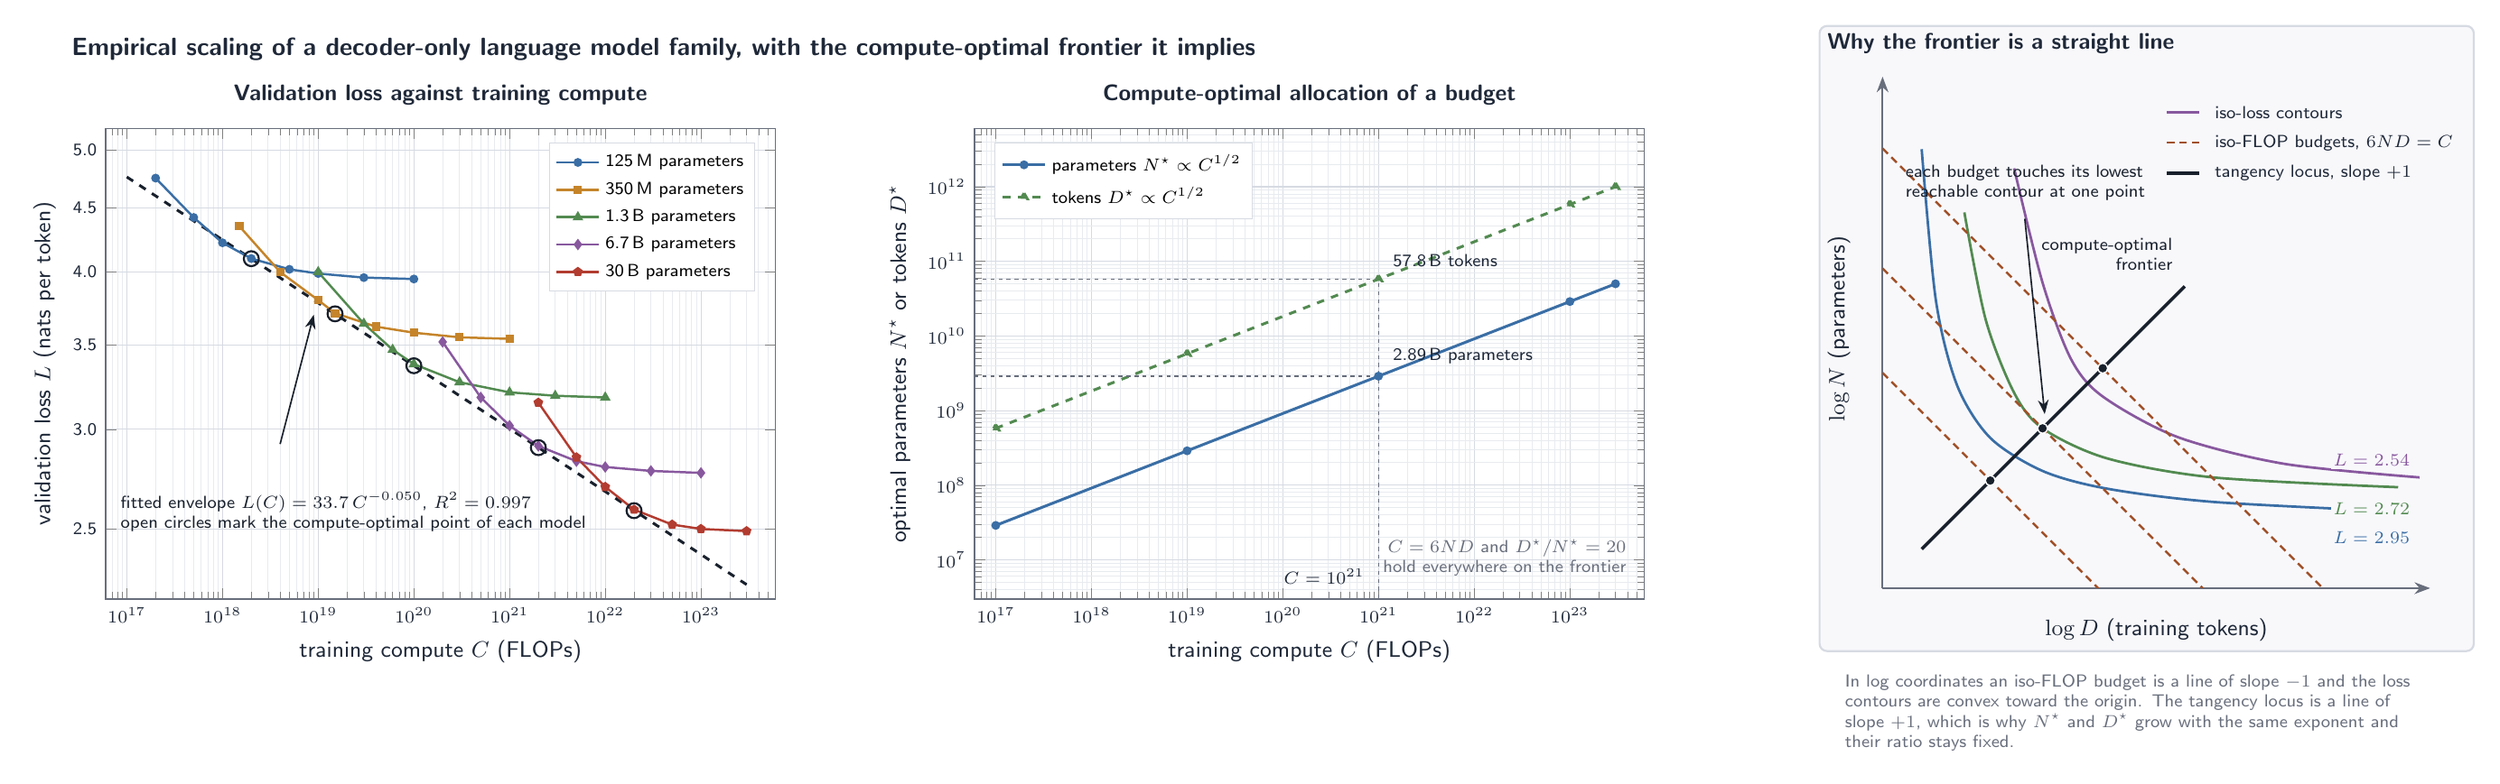
\begin{tikzpicture}[font=\sffamily]

  \begin{loglogaxis}[
      seedaxis,
      name=lossaxis,
      at={(0,0)}, anchor=south west,
      title={Validation loss against training compute},
      xlabel={training compute $C$ (FLOPs)},
      ylabel={validation loss $L$ (nats per token)},
      xmin=6e16, xmax=6e23,
      ymin=2.2, ymax=5.2,
      log basis x=10,
      ytick={2.5,3,3.5,4,4.5,5},
      yticklabels={2.5,3.0,3.5,4.0,4.5,5.0},
      legend pos=north east,
    ]

    \addplot[env,line width=1.1pt,dashed,forget plot] coordinates {
      (1e17,4.760) (1e18,4.243) (1e19,3.781) (1e20,3.370)
      (1e21,3.004) (1e22,2.677) (1e23,2.386) (3e23,2.258)
    };

    \addplot[cA,line width=0.9pt,mark=*,mark size=1.3pt,
             mark options={fill=cA,draw=cA}] coordinates {
      (2e17,4.75) (5e17,4.42) (1e18,4.22) (2e18,4.10)
      (5e18,4.02) (1e19,3.99) (3e19,3.96) (1e20,3.95)
    };
    \addlegendentry{125\,M parameters}

    \addplot[cB,line width=0.9pt,mark=square*,mark size=1.2pt,
             mark options={fill=cB,draw=cB}] coordinates {
      (1.5e18,4.35) (4e18,4.00) (1e19,3.80) (1.5e19,3.71)
      (4e19,3.62) (1e20,3.58) (3e20,3.55) (1e21,3.54)
    };
    \addlegendentry{350\,M parameters}

    \addplot[cC,line width=0.9pt,mark=triangle*,mark size=1.6pt,
             mark options={fill=cC,draw=cC}] coordinates {
      (1e19,4.00) (3e19,3.64) (6e19,3.47) (1e20,3.38)
      (3e20,3.27) (1e21,3.21) (3e21,3.19) (1e22,3.18)
    };
    \addlegendentry{1.3\,B parameters}

    \addplot[cD,line width=0.9pt,mark=diamond*,mark size=1.6pt,
             mark options={fill=cD,draw=cD}] coordinates {
      (2e20,3.52) (5e20,3.18) (1e21,3.02) (2e21,2.91)
      (5e21,2.83) (1e22,2.80) (3e22,2.78) (1e23,2.77)
    };
    \addlegendentry{6.7\,B parameters}

    \addplot[cE,line width=0.9pt,mark=pentagon*,mark size=1.5pt,
             mark options={fill=cE,draw=cE}] coordinates {
      (2e21,3.15) (5e21,2.85) (1e22,2.70) (2e22,2.59)
      (5e22,2.52) (1e23,2.50) (3e23,2.49)
    };
    \addlegendentry{30\,B parameters}

    \addplot[env,only marks,mark=o,mark size=3pt,line width=0.8pt,
             forget plot] coordinates {
      (2e18,4.099) (1.5e19,3.706) (1e20,3.370) (2e21,2.901) (2e22,2.585)
    };

    \node[anchor=west,font=\sffamily\scriptsize,text=env,align=left]
      at (axis cs:7e16,2.58)
      {fitted envelope $L(C) = 33.7\,C^{-0.050}$, $R^2 = 0.997$\\
       open circles mark the compute-optimal point of each model};
    \draw[-{Stealth[length=2mm]},draw=env,line width=0.6pt]
      (axis cs:4e18,2.92) -- (axis cs:9e18,3.70);
  \end{loglogaxis}

  \begin{loglogaxis}[
      seedaxis,
      name=allocaxis,
      at={($(lossaxis.south east)+(28mm,0)$)}, anchor=south west,
      title={Compute-optimal allocation of a budget},
      xlabel={training compute $C$ (FLOPs)},
      ylabel={optimal parameters $N^{\star}$ or tokens $D^{\star}$},
      xmin=6e16, xmax=6e23,
      ymin=3e6, ymax=6e12,
      legend pos=north west,
    ]
    \addplot[cA,line width=1.1pt,mark=*,mark size=1.2pt] coordinates {
      (1e17,2.89e7) (1e19,2.89e8) (1e21,2.89e9) (1e23,2.89e10) (3e23,5.00e10)
    };
    \addlegendentry{parameters $N^{\star} \propto C^{1/2}$}
    \addplot[cC,line width=1.1pt,dashed,mark=triangle*,mark size=1.5pt]
      coordinates {
      (1e17,5.78e8) (1e19,5.78e9) (1e21,5.78e10) (1e23,5.78e11) (3e23,1.00e12)
    };
    \addlegendentry{tokens $D^{\star} \propto C^{1/2}$}

    \node[anchor=south east,font=\sffamily\scriptsize,text=muted,align=right]
      at (axis cs:4.8e23,4.6e6)
      {$C = 6ND$ and $D^{\star}/N^{\star} = 20$\\ hold everywhere on the frontier};

    \draw[draw=muted,line width=0.5pt,dash pattern=on 1.6pt off 1.6pt]
      (axis cs:1e21,3e6) -- (axis cs:1e21,5.78e10);
    \draw[draw=muted,line width=0.5pt,dash pattern=on 1.6pt off 1.6pt]
      (axis cs:6e16,2.89e9) -- (axis cs:1e21,2.89e9);
    \draw[draw=muted,line width=0.5pt,dash pattern=on 1.6pt off 1.6pt]
      (axis cs:6e16,5.78e10) -- (axis cs:1e21,5.78e10);
    \node[anchor=south west,font=\sffamily\scriptsize,text=ink]
      at (axis cs:1.15e21,3.2e9) {2.89\,B parameters};
    \node[anchor=south west,font=\sffamily\scriptsize,text=ink]
      at (axis cs:1.15e21,6.4e10) {57.8\,B tokens};
    \node[anchor=south east,font=\sffamily\scriptsize,text=ink]
      at (axis cs:0.88e21,3.6e6) {$C = 10^{21}$};
  \end{loglogaxis}

  \coordinate (panelorigin) at ($(allocaxis.south east)+(30mm,-2mm)$);

  \begin{scope}[shift={(panelorigin)}]
    \node[draw=grid,line width=0.8pt,rounded corners=3pt,fill=panelfill,
          minimum width=92mm,minimum height=88mm,inner sep=0pt,anchor=south west]
      (panel) at (-0.55,-0.55) {};

    \draw[draw=muted,line width=0.7pt,-{Stealth[length=2.2mm]}]
      (0.35,0.35) -- (0.35,7.55);
    \draw[draw=muted,line width=0.7pt,-{Stealth[length=2.2mm]}]
      (0.35,0.35) -- (8.05,0.35);
    \node[anchor=north,font=\sffamily\small,text=ink] at (4.2,0.05)
      {$\log D$ (training tokens)};
    \node[anchor=south,rotate=90,font=\sffamily\small,text=ink] at (0.02,4.0)
      {$\log N$ (parameters)};

    \begin{scope}
      \clip (0.35,0.35) rectangle (8.05,7.55);

      \draw[draw=cA,line width=1pt,smooth] plot coordinates {
        (0.90,6.53) (1.10,4.40) (1.40,3.20) (1.865,2.465) (2.60,2.00)
        (3.50,1.752) (5.00,1.564) (7.60,1.429)
      };
      \draw[draw=cC,line width=1pt,smooth] plot coordinates {
        (1.50,5.64) (1.80,4.13) (2.20,3.10) (2.60,2.60) (3.50,2.179)
        (5.00,1.909) (7.60,1.771)
      };
      \draw[draw=cD,line width=1pt,smooth] plot coordinates {
        (2.20,6.26) (2.60,4.65) (3.00,3.575) (3.446,3.048) (4.50,2.477)
        (6.00,2.100) (7.90,1.909)
      };

      \draw[draw=isoflop,line width=0.9pt,dash pattern=on 3pt off 2pt]
        (0.35,3.38) -- (3.73,0.0);
      \draw[draw=isoflop,line width=0.9pt,dash pattern=on 3pt off 2pt]
        (0.35,4.85) -- (5.20,0.0);
      \draw[draw=isoflop,line width=0.9pt,dash pattern=on 3pt off 2pt]
        (0.35,6.54) -- (6.89,0.0);

      \draw[draw=env,line width=1.3pt] (0.90,0.90) -- (4.60,4.60);
    \end{scope}

    \foreach \p in {1.865, 2.600, 3.446} {
      \fill[env] (\p,\p) circle (2pt);
      \draw[draw=white,line width=0.5pt] (\p,\p) circle (2pt);
    }

    \node[anchor=west,font=\sffamily\scriptsize,text=cA,fill=panelfill,
          inner sep=1pt] at (6.65,1.06) {$L = 2.95$};
    \node[anchor=west,font=\sffamily\scriptsize,text=cC,fill=panelfill,
          inner sep=1pt] at (6.65,1.47) {$L = 2.72$};
    \node[anchor=west,font=\sffamily\scriptsize,text=cD,fill=panelfill,
          inner sep=1pt] at (6.65,2.15) {$L = 2.54$};

    \draw[draw=cD,line width=1pt] (4.35,7.05) -- (4.80,7.05);
    \node[anchor=west,font=\sffamily\scriptsize,text=ink] at (4.90,7.05)
      {iso-loss contours};
    \draw[draw=isoflop,line width=0.9pt,dash pattern=on 3pt off 2pt]
      (4.35,6.62) -- (4.80,6.62);
    \node[anchor=west,font=\sffamily\scriptsize,text=ink] at (4.90,6.62)
      {iso-FLOP budgets, $6ND = C$};
    \draw[draw=env,line width=1.3pt] (4.35,6.19) -- (4.80,6.19);
    \node[anchor=west,font=\sffamily\scriptsize,text=ink] at (4.90,6.19)
      {tangency locus, slope $+1$};

    \node[anchor=south east,font=\sffamily\scriptsize,text=env,align=right]
      at (4.55,4.70) {compute-optimal\\ frontier};

    \draw[-{Stealth[length=2mm]},draw=env,line width=0.6pt]
      (2.35,5.55) -- (2.63,2.80);
    \node[anchor=south west,font=\sffamily\scriptsize,text=env,align=left,
          text width=36mm] at (0.55,5.68)
      {each budget touches its lowest\\ reachable contour at one point};

    \node[anchor=north west,align=left,font=\sffamily\scriptsize,text=muted,
          text width=80mm] at (-0.30,-0.75)
      {In log coordinates an iso-FLOP budget is a line of slope $-1$ and the
       loss contours are convex toward the origin. The tangency locus is a line
       of slope $+1$, which is why $N^{\star}$ and $D^{\star}$ grow with the
       same exponent and their ratio stays fixed.};

    \node[anchor=south west,font=\sffamily\small\bfseries,text=ink]
      at (-0.55,7.75) {Why the frontier is a straight line};
  \end{scope}

  \node[anchor=north west,font=\sffamily\bfseries,text=ink]
    at ($(lossaxis.north west)+(-6mm,14mm)$)
    {Empirical scaling of a decoder-only language model family, with the
     compute-optimal frontier it implies};

\end{tikzpicture}
\end{document}
